% todo - biologicke pojmy (ale nie vela) definovat hlavne informaticky problem
% obrazok zarovnania - sekvencie, okno, anotacie
% menej slovies - doplnit pri prednasani

% ak budem mať CRF tak porovnanie CRF a HMM - pozret rydzikovu prezentaciu

% Motivacia, ine vysledky
% Ohurit komisiu
% Urobili vela prace, Nebolo to lahke


\documentclass[xcolor=dvipsnames, compress, 12pt]{beamer}
\usepackage[utf8]{inputenc}
\usepackage[slovak]{babel}
\usepackage{lmodern}
\usepackage[T1]{fontenc}
\usepackage{amsfonts}
\usepackage{amssymb}
\usepackage{amsthm}
\usepackage{amsmath}
\usepackage{epsfig}
\usepackage{wrapfig}
\usepackage{caption}
\usepackage{subcaption}
\usepackage{url}
\usepackage{hyperref}
\usepackage{multicol}
\usepackage{fancyvrb}
\usepackage{tabu}
\usepackage{multirow}
\usepackage{booktabs}
\usepackage{regexpatch}
\makeatletter
% Change the `-` delimiter to an active character
\xpatchparametertext\@@@cmidrule{-}{\cA-}{}{}
\xpatchparametertext\@cline{-}{\cA-}{}{}
\makeatother

\usecolortheme[named=Green]{structure}
\usetheme{Madrid}
\setbeamertemplate{navigation symbols}{}
\usebackgroundtemplate{\includegraphics[width=\paperwidth, height=\paperheight]{images/bg.png}}
\setbeamercovered{transparent}

% \setbeamertemplate{footline}[frame number]
% \setbeamertemplate{items}[ball]
% \setbeamertemplate{blocks}[rounded][shadow=true]
% \useoutertheme{umbcfootline}

% \AtBeginSection[]{
% \frame<beamer>{

%     \ifpdf
%       \pdfbookmark[0]{Contents}{toc}
%     \fi
%     \frametitle{Obsah}
%     \setcounter{tocdepth}{2}
%     \tableofcontents[currentsection,subsections,hideothersubsections]

% }
% }

% Show frame number in footbar
\setbeamertemplate{footline}%{miniframes theme}
  {%
    \begin{beamercolorbox}[colsep=1.5pt]{upper separation line foot}
    \end{beamercolorbox}
    \begin{beamercolorbox}[ht=2.5ex,dp=1.125ex,%
      leftskip=.3cm,rightskip=.3cm plus1fil]{author in head/foot}%
      \leavevmode{\usebeamerfont{author in head/foot}\insertshortauthor}%
      \hfill%
      {\usebeamerfont{institute in head/foot}\usebeamercolor[fg]{institute in head/foot}\insertshortinstitute}%
    \end{beamercolorbox}%
    \begin{beamercolorbox}[ht=2.5ex,dp=1.125ex,%
      leftskip=.3cm,rightskip=.3cm plus1fil]{title in head/foot}%
      {\usebeamerfont{title in head/foot}\insertshorttitle} \hfill     \insertframenumber
      % /\inserttotalframenumber %
    \end{beamercolorbox}%
    \begin{beamercolorbox}[colsep=1.5pt]{lower separation line foot}
    \end{beamercolorbox}
  }

% items enclosed in square brackets are optional; explanation below
\title{Zarovnávanie sekvencií\\ s~použitím metód klasifikácie}
\subtitle{
\vspace{0.5cm}
\small Diplomová práca
}
\author[Michal Hozza]{\small Bc. Michal Hozza \\ \vspace{1cm} \footnotesize \textbf{Vedúci práce:} Mgr. Tomáš Vinař, PhD. \\ \textbf{Konzultant:} Mgr. Michal Nánási\\ \vspace{.5cm}}
\institute[FMFI UK \insertshortdate]{
  Fakulta matematiky, fyziky a informatiky,
  Univerzita Komenského, Bratislava\\
}
\date[\the\year]{\footnotesize 17.6.2014}

\newcommand{\lenitem}[2][.6\linewidth]{\parbox[t]{#1}{\strut #2\strut}}

\newtheorem{vt}{Veta}[section]
\newtheorem{lema}[vt]{Lema}
\theoremstyle{definition}
\newtheorem{df}[vt]{Definícia}

\begin{document}

%--- the titlepage frame -------------------------%
\begin{frame}[plain]
  \titlepage
\end{frame}

%--- the presentation begins here ----------------%

\begin{frame}{Obsah}
  \transdissolve[duration=0.1]
  % \begin{multicols}{2}
  \tableofcontents
  % \end{multicols}
\end{frame}


\section{Úvod}

\subsection{Zarovnávanie sekvencií}
\begin{frame}[fragile]{Zarovnávanie sekvencií}
  \begin{itemize}
      % \item DNA sekvencia je reťazec, ktorý sa skladá z jednotlivých báz: adenín (A), guanín (G), cytozín (C) a tymín (T)
      \item jedným zo základných bioinformatických problémov
      \item identifikuje časti sekvencie, ktoré vznikli z~toho istého predka (zarovnané bázy), inzercie a delécie v~priebehu evolúcie (medzery v~zarovnaní)
  \end{itemize}
\pause
Príklad:
  \begin{Verbatim}[commandchars=\\\{\}]
 \textcolor{Blue}{GT}\textcolor{Red}{G}\textcolor{Blue}{GACCGTT}\textcolor{Green}{------}\textcolor{Red}{C}\textcolor{Blue}{CTT}\textcolor{Red}{CCG}\textcolor{Blue}{GCAATCA}\textcolor{Red}{C}\textcolor{Blue}{G}\textcolor{Green}{AGA}\textcolor{Blue}{AA}\textcolor{Red}{AG}\textcolor{Blue}{CCAC}\textcolor{Red}{G}\textcolor{Blue}{T}
 \textcolor{Blue}{GT}\textcolor{Red}{C}\textcolor{Blue}{GACCGTT}\textcolor{Green}{TCAGTG}\textcolor{Red}{A}\textcolor{Blue}{CTT}\textcolor{Red}{GAA}\textcolor{Blue}{GCAATCA}\textcolor{Red}{G}\textcolor{Blue}{G}\textcolor{Green}{---}\textcolor{Blue}{AA}\textcolor{Red}{CA}\textcolor{Blue}{CCAC}\textcolor{Red}{C}\textcolor{Blue}{T}
  \end{Verbatim}
\end{frame}

\begin{frame}[fragile]{Zarovnávanie sekvencií ako informatický problém}
\begin{itemize}
  \item Vstupom sú dve sekvencie $X = x_1x_2\dots x_n$ a $Y = y_1y_2\dots y_m$
  \item Výstupom je zarovnanie sekvencií, ktoré má najvyššie možné skóre podľa danej skórovacej schémy
  \item Skórovacia schéma môže byť napr. $+1$ za zhodu a $-1$ za medzeru alebo nezhodu
  \item V tomto prípade sa dá najlepšie zarovnanie nájsť v čase $O(nm)$ dynamickým programovaním
  \item V praxi sa používajú zložitejšie schémy, v našej práci používame párové HMM
\end{itemize}
\end{frame}

\begin{frame}{Párové Skryté Markovovské modely (pHMM)}
   \begin{itemize}
    \item pravdepodobnostný model inšpirovaný konečnými automatmi

    \begin{df}[pHMM]
        pHMM je 6-ica $(K, \Sigma_X, \Sigma_Y, \pi, a, e)$, kde $K$ je množina stavov, $\Sigma_X$ je množina symbolov $X-ovej$ sekvencie, $\Sigma_Y$ je množina symbolov $Y-ovej$ sekvencie, $\pi = \{\pi_i\}_{i \in K}$ je distribúcia začiatočných stavov, $a = \{a_{i,j}\}_{i, j \in K}$ je distribúcia prechodov a $e = \{e_{i,x,y}\}_{i\in K,\, x\in \Sigma_X \cup \{\varepsilon\},\, y\in \Sigma_Y \cup \{\varepsilon\}}$ je distribúcia emisií.
    \end{df}

    \item narozdiel od jednoduchého HMM generuje dve sekvencie, pričom môže mať stavy, ktoré generujú symboly v oboch sekvenciách, alebo len v jednej zo sekvencií
    % \item ,,pomlčky'' môže vložiť na ľubovoľné miesto (to v jednoduchom HMM nie je možné)
  \end{itemize}

\end{frame}


\begin{frame}{Párové Skryté Markovovské modely (pHMM)}
  Príklad: pHMM pre zarovnávanie sekvencií
  \begin{itemize}
      \item $K = \{M, X, Y\},\, \Sigma_X = \Sigma_Y = \{A, C, G, T\}$
      \item M \textit{(Match)} -- emituje dvojice báz: $AA, AC, AG,\dots, TT$
      \item X \textit{(Insert X)} a Y \textit{(Insert Y)} -- emitujú jednotlivé bázy: $A,C,G,T$
  \end{itemize}
  \begin{center}
  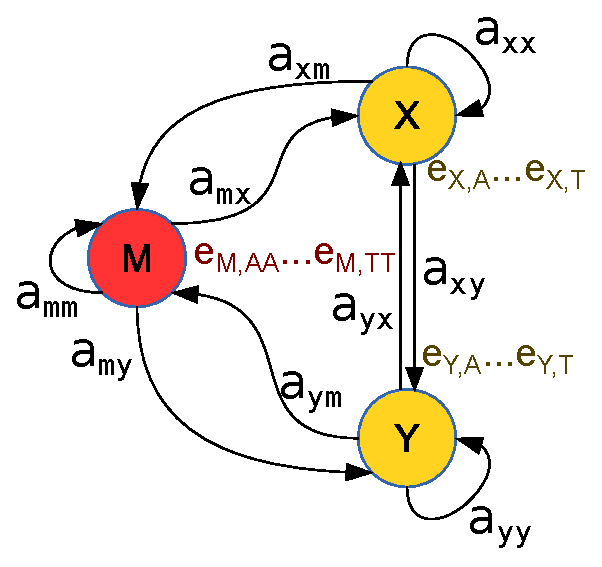
\includegraphics[width=.30\textwidth]{images/simple_model}
  \end{center}
\end{frame}

\begin{frame}[fragile]{Párové Skryté Markovovské modely (pHMM)}
  \begin{itemize}
      \item Postupnosť stavov definuje konkrétne zarovnanie vstupných sekvencií
      \item Pri zarovnávaní hľadáme najpravdepodobnejšiu postupnosť stavov (pomocou Viterbiho algoritmu)
  \end{itemize}
  \pause
   Príklad:
  \begin{itemize}
  \item Vstupné sekvencie
  \begin{verbatim}
  GTGGACCGTTCCTTCCGGCAATCACGAGAAAAGCCACGT
  GTCGACCGTTTCAGTGACTTGAAGCAATCAGGAACACCACCT
  \end{verbatim}
  \item Jedno z možných zarovnaní spolu so stavmi
  \begin{Verbatim}[commandchars=\\\{\}]
  GTGGACCGTT------CCTTCCGGCAATCACGAGAAAAGCCACGT
  \textcolor{Red}{MMMMMMMMMM}\textcolor{YellowOrange}{YYYYYY}\textcolor{Red}{MMMMMMMMMMMMMMMM}\textcolor{YellowOrange}{XXX}\textcolor{Red}{MMMMMMMMMM}
  GTCGACCGTTTCAGTGACTTGAAGCAATCAGG---AACACCACCT
  \end{Verbatim}
  \end{itemize}
\end{frame}

\begin{frame}[fragile]{Zarovnávanie sekvencií s anotáciou}
\begin{itemize}
  \item máme k dispozícii anotácie k sekvenciám (napr. gén/negén)
  \item anotácia môže byť aj komplexnejšia -- pozostávajúca z rôznych indikátorov, pochádzajúcich z biologických experimentov
  \item to nám môže pomôcť lepšie určiť biologicky korektné zarovnanie
  \end{itemize}
  \pause
  Príklad:
  \begin{itemize}
  \item S anotáciou
 \begin{Verbatim}[commandchars=\\\{\}]
  \textcolor{Green}{0000000      }\textcolor{Blue}{111111111111111111111}\textcolor{Green}{00000000000}
  GTGGACC------\textcolor{Red}{GTT}CCTTCCGGCAATCACGAGAAAAGCCACGT
  GTCGACCGTTTCAGTGACTTGAAGCAATCAGG\textcolor{Red}{AA}---CACCACCT
  \textcolor{Green}{0000000000000}\textcolor{Blue}{111111111111111111111   }\textcolor{Green}{00000000}
  \end{Verbatim}
  \item Bez anotácie
  \begin{Verbatim}[commandchars=\\\{\}]
  GTGGACC\textcolor{Red}{GTT}------CCTTCCGGCAATCACGAGAAAAGCCACGT
  GTCGACCGTTTCAGTGACTTGAAGCAATCAGG---\textcolor{Red}{AA}CACCACCT
  \end{Verbatim}
\end{itemize}
\end{frame}

% \section{Modely a Existujúce riešenia}
% \subsection{Modely}
% \begin{frame}{Modely}
% Generatívny:
% \begin{itemize}
% \item sa snaží modelovať proces, ktorý generuje dáta ako pravdepodobnosť $P(X,Y,Z)$
% \item rozložíme ju pomocou nezávislých predpokladov na procese $\longrightarrow$ obmedzujúce
% \end{itemize}
% \pause
% Diskriminačný
% \begin{itemize}
% \item priamo odhaduje $P(Z|X,Y)$ alebo prislúchajúcu diskriminačnú funkciu, a preto sa zamerá na podstatnú časť problému odhadu
% \item Nepotrebuje nezávislosť $\longrightarrow$ silnejšie
% \end{itemize}
% \end{frame}

% % ToDo - lepsie popisat existujuce modely
% \subsection{Príbuzné témy}
% \begin{frame}{Príbuzné témy (existujúce riešenia)}
%   \begin{itemize}
%     \item Problém inverzného zarovnania
%     \pause
%     \item Support vector training of protein alignment models
%     \begin{itemize}
%       \item Support Vector Machine (SVM)
%       \item Umožňuje trénovať pomocou rôznych účelových funkcií
%     \end{itemize}
%     \pause
%     \item Contralign: Discriminative training for protein sequence alignment.
%     \begin{itemize}
%       \item Conditional Random Fields (CRF)
%       \item Neumožnuje trénovať pomocou rôznych účových funkcií
%     \end{itemize}
%   \end{itemize}
% \end{frame}

% \section{Naše riešenia}
% \subsection{Odlišnosti nášho riešenia}
% \begin{frame}{Odlišnosti nášho riešenia}
%   \begin{itemize}
%     \item Korekcia existujúcich zarovnaní
%     \begin{itemize}
%       \item Použitie súbežne s~existujúcimi zarovnávačmi
%     \end{itemize}
%     \pause
%     \item Rôzne modely využitia klasifikátora
%     \pause
%     \item Rôzne metódy trénovania
%     \pause
%     \item Možnosť učenia bez učiteľa
%     \pause
%     \item Iný klasifikátor
%     \begin{itemize}
%       \item možno porovnanie viac rôznych klasifikátorov
%       \item pípadne abstrakcia od klasifikátora
%     \end{itemize}
%   \end{itemize}
% \end{frame}

%ToDo: Obrázok
% \section{Existujúce riešenia}
% \begin{frame}{Existujúce metódy zarovnávania sekvencií s dodatočnou informáciou}
%   \begin{df}[Problém inverzného zarovnania]
%   Vstupom sú dve sekvencie $X$, $Y$ a ich zarovnanie $Z$.
%   Výstupom sú parametre, podľa ktorých je toto zarovnanie optimálne.
%   \end{df}
%   \pause
%   \begin{itemize}
%     \item doterajšie publikácie boli o zarovnávaní proteínových sekvencií
%     \item doterajší výskum sa zaoberal havne riešením problému IZ
%     \item v \cite{svmTrainingProteinsAlignment} využili SVM na nájdenie parametrov a použili anotáciu o štruktúre sekvencií
%     \item podobný prístup zvolili v \cite{contralign}, kde na nájdenie parametrov využili CRF
%     \pause
%     \item obe riešenia ťažia z výhod diskriminatívneho učenia, kde hľadáme $P(Z|W)$ (namiesto $P(Z,W)$, ktoré hľadáme pri generatívnych modeloch)
%   \end{itemize}
% \end{frame}

\subsection{Ciele práce}
\begin{frame}{Ciele práce}
  \begin{itemize}
  \item cieľom práce je vytvoriť nové metódy na korekciu zarovnaní biologických sekvencií na základe prídavnej informácie
  \item integrácia tejto informácie bude zabezpečená pomocou techník využívaných na klasifikáciu v~strojovom učení
  \end{itemize}
  \vspace{.5cm}
  \pause
  \begin{itemize}
  \item vzhľadom ku komplexnosti pridanej informácie, je veľmi ťažké systematickým spôsobom zakomponovať anotáciu do skórovacích schém založených na pHMM
  \item modelovanie takejto informácie v rámci pHMM by bolo neefektívne
  \end{itemize}
\end{frame}


\section{Naše riešenie}
\begin{frame}{Zhrnutie nášho riešenia}
  \begin{enumerate}
    \item informáciu zosumarizujeme do jedného čísla
    \begin{itemize}
      \item pre pár pozícií $(i, j)$ chceme číslo $S(i, j)$, ktoré na základe lokálnej informácie vyjadruje, ako dobre k sebe príslušné pozície pasujú
      \item to je vhodná úloha pre klasifikátory
    \end{itemize}
    \item navrhneme systematický spôsob, ako toto číslo zakomponovať do skórovacej schémy pHMM
  \end{enumerate}
\end{frame}

% \begin{frame}{Naše riešenie -- odlišnosti}
%   \begin{itemize}
%     \item naše modely sú kombináciou generatívneho a diskriminačného prístupu
%     \item naše modely sú založené na pHMM
%     \item používame dva rôzne klasifikátory
%     \item architektúry našich modelov abstrahujú od klasifikátora
%     \item ako klasifikátor sme použili \emph{náhodný les (angl. Random forest)} \cite{randomForestPaper}
%     \item zaoberáme sa DNA sekvenciami, nie proteínmi
%     \item nemáme k~dispozícii sekundárnu štruktúru, ale iný typ anotácií
%   \end{itemize}
% \end{frame}

\subsection{Klasifikácia na základe lokálnej informácie}

\begin{frame}{Klasifikácia na základe lokálnej informácie}
\begin{itemize}
  \item anotácie sme zakomponovali pomocou dvoch typov klasifikátorov
  \begin{enumerate}
    \item Match -- rozhoduje či dané pozície majú byť zarovnané k~sebe
    \item Indel -- rozhoduje či daná pozícia má byť zarovnaná k medzere
  \end{enumerate}
  \item výstup $\in \left<0,1\right>$ -- istota klasifikátora, že dané dve pozície majú byť zarovnané k~sebe (v~Indel klasifikátore, že daná pozícia má  byť zarovnaná k~medzere)
  \item atribúty sú okná veľkosti $w$
\end{itemize}
\end{frame}

\begin{frame}{Okno pre klasifikátor}
\begin{figure}[h]
        \centering
        \begin{subfigure}[b]{0.35\textwidth}
                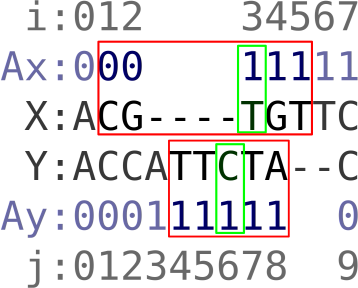
\includegraphics[width=\textwidth]{images/window_m}
                \caption{Match klasifikátor}
                \label{fig:window-m}
        \end{subfigure}%
        \qquad\qquad %add desired spacing between images, e. g. ~, \quad, \qquad etc.
          %(or a blank line to force the subfigure onto a new line)
        \begin{subfigure}[b]{0.35\textwidth}
                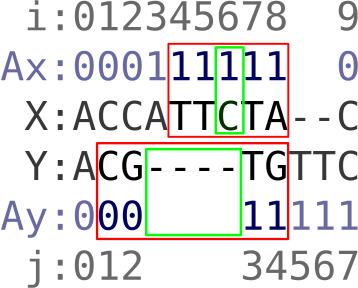
\includegraphics[width=\textwidth]{images/window_i}
                \caption{Indel klasifikátor}
                \label{fig:window-i}
        \end{subfigure}
        \caption[Okno klasifikátora]{Okno klasifikátora pre pozície $i = 6$ a $j = 3$}
\end{figure}
\end{frame}

\begin{frame}{Klasifikácia na základe lokálnej informácie}
  \begin{itemize}
    \item k~dátam sme pridali informácie o~zhodách na zodpovedajúcich pozíciách, čím sa nám podarilo vylepšiť úspešnosť klasifikátora
    \item úspešnosť Match klasifikátora: \textbf{89,87\%}
    \item úspešnosť Indel klasifikátora: \textbf{81,78\%}
    \item klasifikátor sa dokáže naučiť, ktoré okná majú byť zarovnané k~sebe a ktoré nie
\end{itemize}
\end{frame}


\begin{frame}{Úspešnosť klasifikátora}
\begin{figure}[h]
        \centering
        \begin{subfigure}[b]{0.45\textwidth}
               \includegraphics[width=\textwidth]{images/randomforest_combined_5_test}
                \caption{Match klasifikátor}
        \end{subfigure}
        \qquad
        \begin{subfigure}[b]{0.45\textwidth}
                \includegraphics[width=\textwidth]{images/randomforest_combined_5_indel_test}
                \caption{Indel klasifikátor}
        \end{subfigure}
        \caption{Distribúcia výstupu klasifikátora pre pozitívne a negatívne príklady.}
\end{figure}
\end{frame}


\begin{frame}{Dôležitosť atribútov}
\begin{figure}[h]
        \centering
        \begin{subfigure}[b]{0.45\textwidth}
                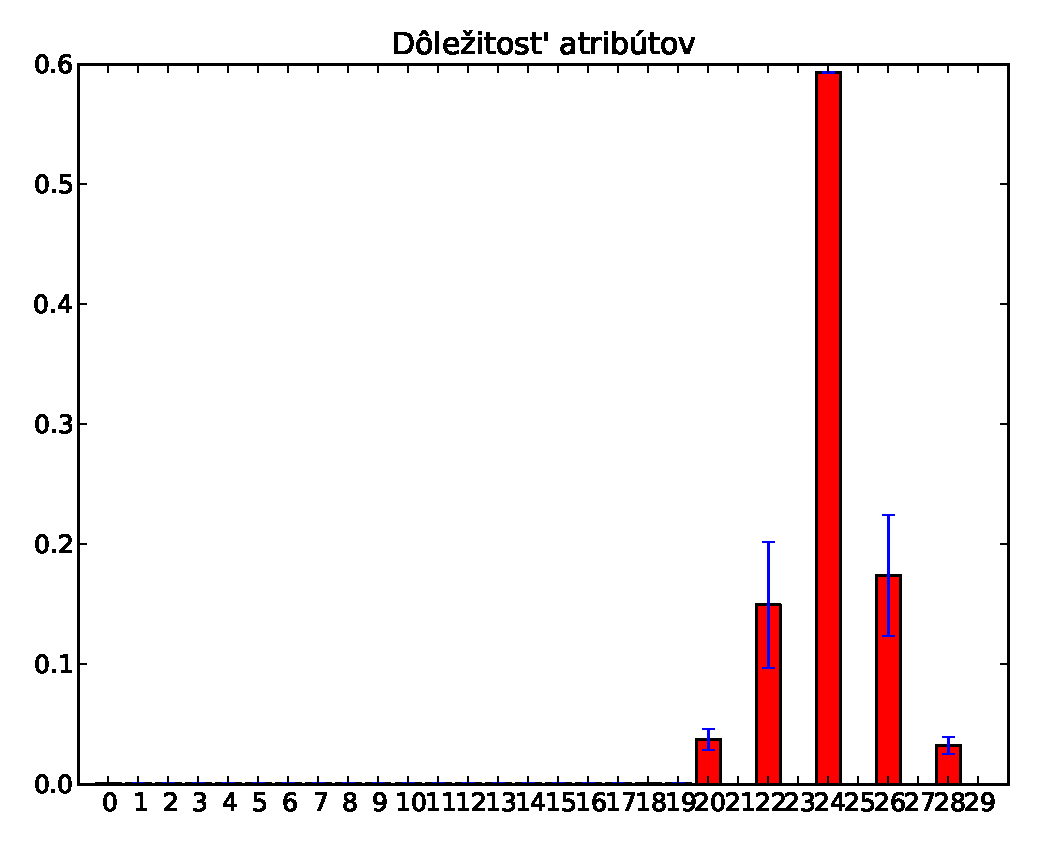
\includegraphics[width=\textwidth]{images/randomforest_combined_5_bars}
                \caption{Match klasifikátor}
        \end{subfigure}
        \qquad
        \begin{subfigure}[b]{0.45\textwidth}
                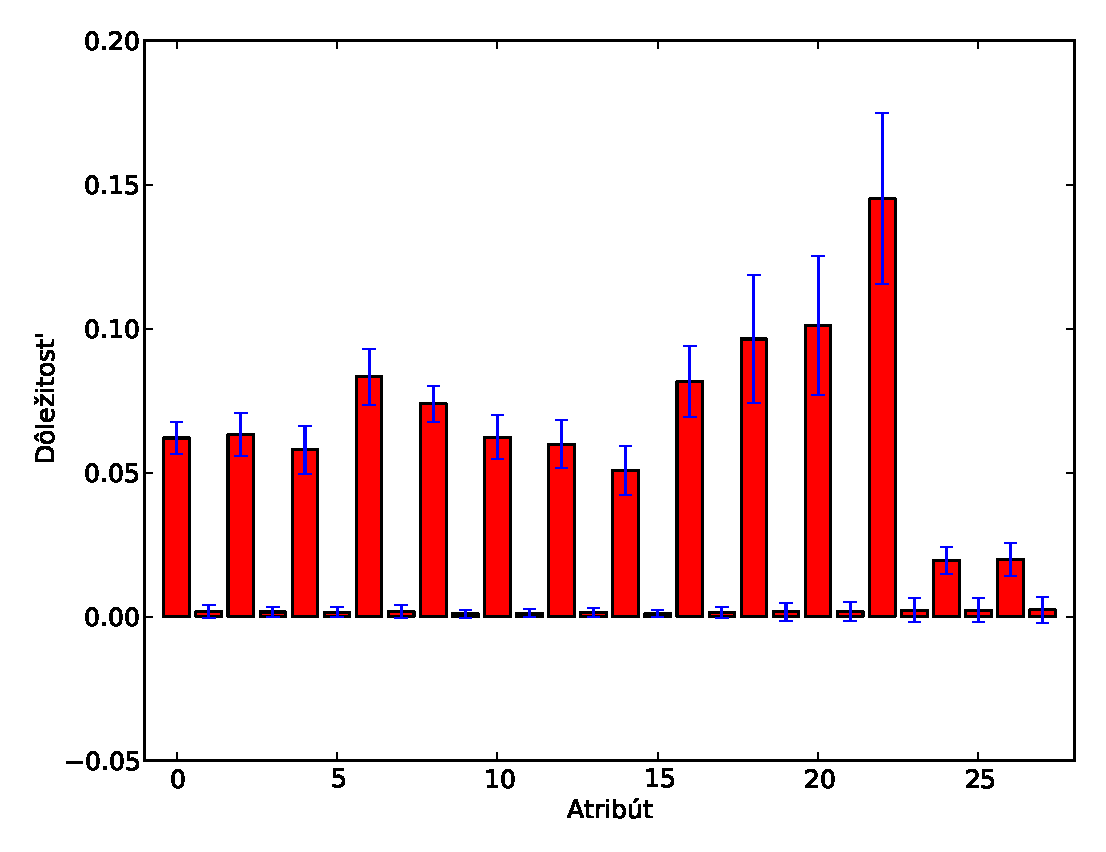
\includegraphics[width=\textwidth]{images/randomforest_combined_5_indel_bars}
                \caption{InDel klasifikátor}
        \end{subfigure}
        \caption{Dôležitosť atribútov v~klasifikátore.}
\end{figure}
\end{frame}

\subsection{Zakomponovanie výsledkov klasifikácie do pHMM}
\begin{frame}{Zakomponovanie výsledkov klasifikácie do pHMM}

\begin{itemize}
  \item skonštruovali sme dva modely pre zarovnanie sekvencií s~anotáciami za pomoci klasifikátora
  \begin{enumerate}
    \item Model s~klasifikátorom ako emisiou
    \item Model s~klasifikátorovou páskou
  \end{enumerate}
  \item založené na párových skrytých Markovovských modeloch.
\end{itemize}

\end{frame}

\begin{frame}{Model s klasifikátorom ako emisiou (Model A)}
  \mbox{}\hfill\raisebox{-\height}[0pt][0pt]{
   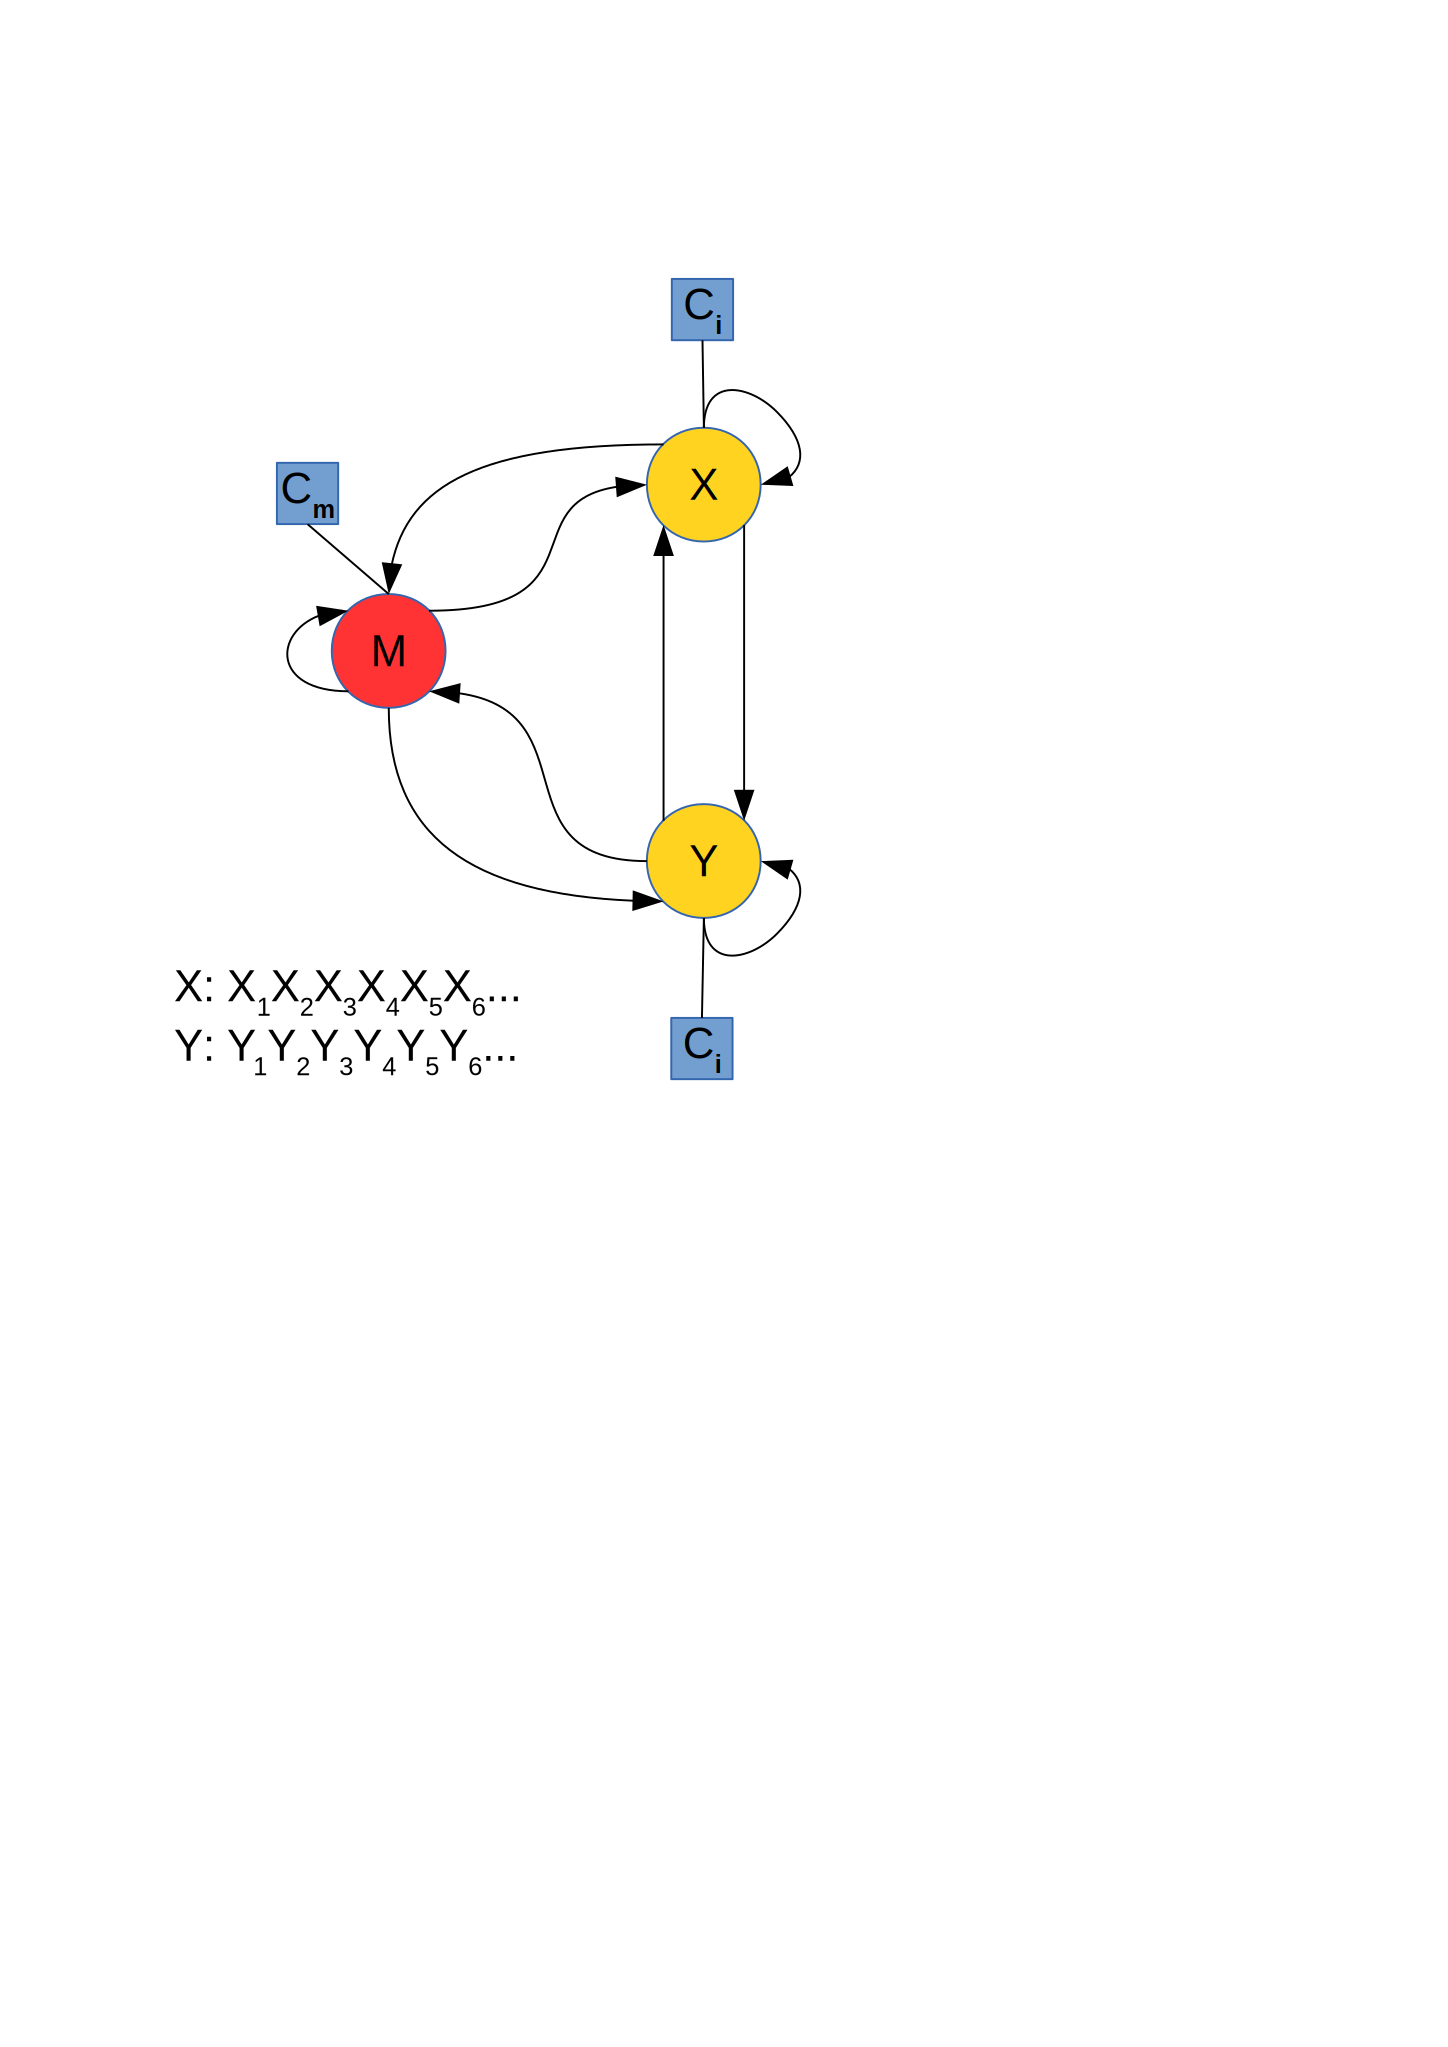
\includegraphics[width=.30\textwidth]{images/zakladny_model}
   }
  \vspace*{-\baselineskip}

  \begin{itemize}
    \item \lenitem{emisné tabuľky stavov nahradíme výstupom z~klasifikátora}
    \item \lenitem{model nie je korektný pravdepodobnostný model, pretože výstupy klasifikátora nesčitujú do~1}
    \item \lenitem{prechodové pravdepodobnosti sme natrénovali zo zarovnaní z~trénovacej vzorky}
  \end{itemize}
\end{frame}

\begin{frame}{Model s~klasifikátorovou páskou (Model B)}
  \mbox{}\hfill\raisebox{-\height}[0pt][0pt]{
   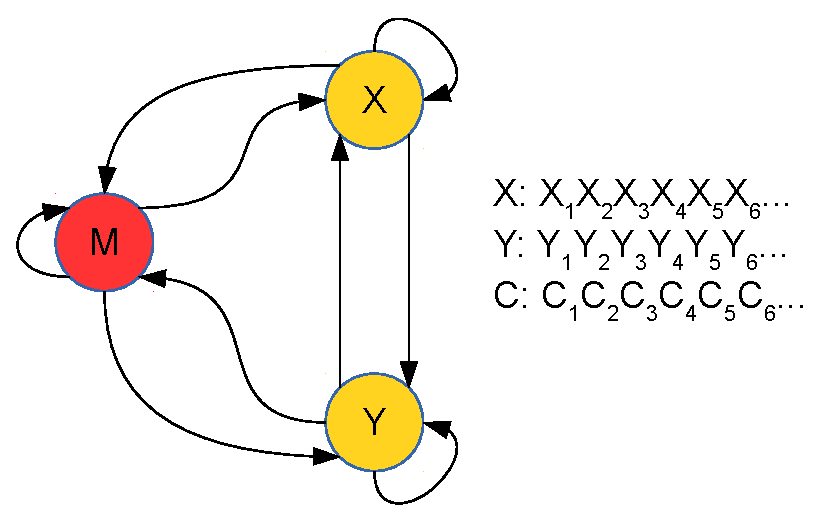
\includegraphics[width=.30\textwidth]{images/model_clf_paska}
   }
  \vspace*{-\baselineskip}

  \begin{itemize}
      \item \lenitem{modelujeme navyše sekvenciu výstupov klasifikátora vo forme pásky}
      \item \lenitem{trénujeme všetky parametre na trénovacej vzorke zarovnaní obohatenej o~pásku s~výstupmi z~klasifikátora}
  \end{itemize}

  \begin{itemize}
    \item \lenitem{páska je cesta v~2D tabuľke výstupov klasifikátorov}
    \item \lenitem{zhoduje sa s~cestou zarovnania}
    \item ak sa pohneme horizontálne, alebo vertikálne, používame Indel klasifikátor a ak sa pohneme diagonálne, tak použijeme Match klasifikátor
  \end{itemize}
\end{frame}

\begin{frame}[fragile]{Klasifikátorová páska}
\begin{figure}[htp]
    \centering
    \begin{subfigure}[m]{0.5\textwidth}
    \centering
    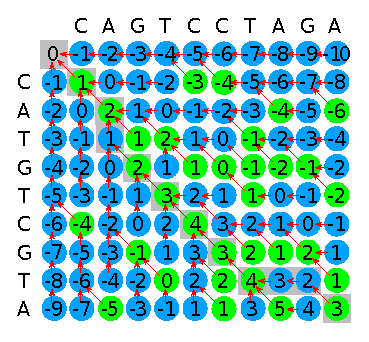
\includegraphics[width=\textwidth]{images/clf_tape}
    \end{subfigure}
    ~
    \begin{subfigure}[m]{0.3\textwidth}
    \centering
    \begin{BVerbatim}[commandchars=\\\{\}]
    CATGTCAT--A
    CA-GTCCTAGA
    {\color{green}MM}{\color{blue}I}{\color{green}MMMMM}{\color{blue}II}{\color{green}M}
    \end{BVerbatim}
    \end{subfigure}
    \caption{Použité klasifikátory v~klasifikátorovej páske}
    \label{fig:clf-tape}
\end{figure}
\end{frame}



\section{Výsledky}
\begin{frame}{Výsledky}

\begin{table}[htp]
\footnotesize
% \catcode`\-=12
\centering
\begin{tabu} to \textwidth {X[l]X[c]X[c]X[c]X[c]X[c]X[c]X[c]X[c]}
\toprule
\multirow{2}{*}{Dáta} &
\multicolumn{2}{c}{Model A} &
\multicolumn{2}{c}{Model B } &
\multicolumn{2}{c}{Ref. Model } &
\multicolumn{2}{c}{Muscle} \\
\cmidrule(r){2-3}\cmidrule(lr){4-5}\cmidrule(lr){6-7}\cmidrule(l){8-9}
& Zhoda & Tranz. & Zhoda & Tranz. & Zhoda & Tranz. & Zhoda & Tranz.\\
\midrule
sim1 & 79,75\% & 44,97\% & 84,35\% & 56,5\% & \textbf{85,78\%} & \textbf{61,03\%} & 82,72\%& 58,76\%\\
sim2 & 70,14\% & --- & \textbf{71,47}\% & --- & 60,38\% & --- & 61,47\% & --- \\
bio & \textbf{91,40\%} & 96,63\% & 91,24\% & \textbf{96,89\%} & 91,34\% & 96,45\% & 91,28\% & 95,98\%\\
\bottomrule
\end{tabu}
\caption[Porovnanie s~existujúcimi zarovnávačmi]{Porovnanie našich modelov s~referenčným modelom a zarovnávačom muscle.}
\label{tab:success-compare}
\end{table}
\begin{itemize}
    \item Tranzitivitu počítame z troch zarovnaní $AB, BC$ a $AC$, ako percentuálnu zhodu medzi zložením prvých dvoch zarovnaní ($AB \circ BC$) a tretieho zarovnania $AC$.
\end{itemize}
\end{frame}



% \begin{frame}{Výsledky}
% \begin{table}[htp]
% \footnotesize
% % \catcode`\-=12
% \centering
% \begin{tabu} to \textwidth {X[l]X[c]X[c]X[c]X[c]X[c]X[c]X[c]X[c]}
% \toprule
% \multirow{2}{*}{Dáta} &
% \multicolumn{2}{c}{Model A} &
% \multicolumn{2}{c}{Model B } &
% \multicolumn{2}{c}{Ref. Model } &
% \multicolumn{2}{c}{Muscle} \\
% \cmidrule(r){2-3}\cmidrule(lr){4-5}\cmidrule(lr){6-7}\cmidrule(l){8-9}
% & Zhoda & Tranz. & Zhoda & Tranz. & Zhoda & Tranz. & Zhoda & Tranz.\\
% \midrule
% sim1 & 20,25\% & 55,03\% & 15,65\% & 43,5\% & \textbf{14,22\%} & \textbf{38,97\%} & 17,28\%& 41,24\%\\
% sim2 & 29,86\% & --- & \textbf{28,53}\% & --- & 39,62\% & --- & 38,53\% & --- \\
% bio & \textbf{8,6\%} & 3,37\% & 8,76\% & \textbf{3,11\%} & 8,66\% & 3,55\% & 8,72\% & 4,02\%\\
% \bottomrule
% \end{tabu}
% \caption{Porovnanie \textit{chyby} našich modelov s~referenčným modelom a zarovnávačom muscle.}
% \label{tab:success-compare}
% \end{table}
% \end{frame}

\section{Záver}
\begin{frame}{Záver}
  \begin{itemize}
    \item navrhli sme spôsob zakomponovania dodatočnej informácie do zarovnávania sekvencií
    \item vytvorili sme vhodnú sadu atribútov pre klasifikátory
    \item vytvorili sme dva modely, ktoré zahŕňajú výstup klasifikátora do zarovnania
    \item úspešne sme implementovali zarovnávač s dodatočnou informáciou
    \begin{itemize}
      \item naše riešenie je ľahko rozšíriteľné (umožnuje pridanie nových modelov, sady atribútov, výmenu klasifikátora \dots)
    \end{itemize}
    \item podarilo sa nám prekonať úspešnosť referenčných zarovnávačov bez anotácie na biologických dátach
  \end{itemize}
\end{frame}

\section{}

\begin{frame}[plain, c]
  \transdissolve[duration=5]
  \begin{center}
  \textbf{\color{Green} \LARGE Ďakujem za pozornosť!}

  \vspace{1cm}

  
\includegraphics[width=.30\textwidth]{images/realigner}

  \vspace{.5cm}

  \url{https://github.com/mhozza/realigner}
  \end{center}

\end{frame}

%-------------------------------------------

% \begin{frame}{Todo}
%   Todo
% \end{frame}

\begin{frame}{Čo považujeme za heuristiku?}
\begin{itemize}
  \item Algoritmy, ktoré hľadajú optimálne zarovnanie vzhľadom na nejakú skórovaciu schému a vždy ho nájdu nepovažujeme za heuristické. Takýmto algoritmom je aj Viterbiho algoritmus, ktorý používame v našej práci. Skórovacia schéma je v našom prípade pHMM s klasifikátorom.
  \item Okrem toho existujú rôzne heuristické algoritmy, ktoré pracujú rýchlejšie za cenu nenájdenia optimálneho zarovnania.
  \end{itemize}
\end{frame}

\begin{frame}{Dôvody pre výber klasifikátora Náhodný les}
\begin{itemize}
  \item V práci sme sa nezaoberali porovnaním rôznych klasifikačných algoritmov
  \item Namiesto toho sme implementovali zarovnávač, v ktorom je možné jednoducho klasifikátor vymeniť za iný
  \item Za najlepší tento klasifikátor považujú jeho autori v článku \cite{randomForestPaper}
  \item Nás zaujímalo hlavne to, že funguje dostatočne dobre, a že je rýchly
  \item V rámci pokusov sme vyskúšali aj algoritmus SVM (dosahoval značne horšiu úspešnosť a bol pomalý) a rôzne stromové algoritmy (dosahovali podobnú úspešnosť aj rýchlosť trénovania)
  \item Z dôvodu časovej náročnosti detailnejších experimentov sme takéto porovnanie nezahrnuli do našej práce
\end{itemize}
\end{frame}

\begin{frame}{Trénovanie náhodných lesov}
\begin{itemize}
  \item V práci sme si zaviedli dva typy listov -- uzavretý a otvorený
  \item Uzavretý má priradenú triedu, otvorený nie. Jediný list na začiatku je otvorený (pokiaľ neobsahuje len dáta jednej triedy)
  \item List uzavrieme a priradíme mu triedu, ak všetky dáta v tomto liste patria do tej triedy. Keďže ide učenie s učiteľom, príslušnosť dát do danej triedy poznáme.
  \item Dátovú sadu, pre každý strom v lese, získame náhodným výberom $N$ vektorov s opakovaním z danej trénovacej sady veľkosti $N$.
  \item Druhý prvok náhodnosti spočíva v tom, že v každom vrchole sa vyberie len malá podmnožina atribútov, z ktorých sa vyberá najinformatívnejší atribút
  \item Časť dát z globálnej sady sa nám v danej množine nevyskytne. Tieto dáta sú tzv. \textit{out of bag} a OOB chyba je chyba počítaná na týchto dátach.
\end{itemize}
\end{frame}


\begin{frame}{Klasifikátory vs. modely}
\begin{itemize}
  \item v našich modeloch máme tri stavy dvoch typov -- jeden Match stav a dva Insert stavy
  \item Match stav používa Match klasifikátor a Insert stavy používajú Indel klasifikátor
\end{itemize}
\end{frame}


\begin{frame}{DNA vs. proteíny}
\begin{itemize}
  \item z hľadiska modelov a algoritmov, medzi DNA a proteínmi nie je rozdiel
  \item rozdiel je vo vlastnostiach sekvencie a v dostupných anotáciách
  \item časť DNA (gény) kóduje proteíny, preto sa na zarovnávanie proteínov môžme pozerať ako na podproblém zarovnávania DNA.
\end{itemize}


\end{frame}



%-------------------------------------------

\begin{frame}[allowframebreaks]{Literatúra}
  \bibliographystyle{apalike}
  \bibliography{references}
\end{frame}


\end{document}
